\section{基于CycleGAN网络改进的去雾还原算法\label{方法A}}

随着深度学习技术的飞速发展,生成对抗网络(GAN)及其变体在图像生成和转换领域取得了显著成果。去雾还原作为计算机视觉中的关键任务之一,旨在从有雾图像中恢复出清晰、无雾的图像,对于提高图像质量、增强视觉效果以及辅助后续的图像分析任务具有重要意义。CycleGAN 作为一种新兴的无监督图像到图像转换方法,在去雾还原算法中展现出巨大潜力。

生成对抗网络(GAN)由 Goodfellow 等人于 2014 年提出,其核心思想是通过两个神经网络——生成器(Generator)和判别器(Discriminator)的对抗训练来生成逼真的数据。生成器的目标是将随机噪声映射到目标数据分布,以生成尽可能真实的样本;判别器则负责区分生成样本和真实样本。在训练过程中,生成器和判别器不断竞争,生成器努力欺骗判别器,使其无法区分生成样本和真实样本,而判别器则努力提高自己的辨别能力。最终,理想情况下生成器能够生成以假乱真的样本,判别器则无法有效区分真假样本。

然而,GAN 在实际应用中存在一些局限性。首先,GAN 的训练过程较为复杂且不稳定,容易出现模式崩溃(Mode Collapse)问题,即生成器只能生成有限类型的样本,无法覆盖数据分布的多样性。其次,GAN 需要大量的成对数据进行训练,这在许多实际场景中难以获取,限制了其应用范围。

基于 CycleGAN 的改进去雾算法作为新一代无监督去雾方法,通过多尺度残差生成器设计、局部 - 全局判别器架构及空间自注意机制三大核心创新,显著提升了去雾图像的质量与真实性。本文基于改进 CycleGAN 网络,针对实际场景中因光照变化复杂、雾气类型多样及场景语义丰富导致的去雾效果不理想问题,提出针对性优化方案。本章将系统性阐述改进 CycleGAN 网络的核心架构设计及其在复杂场景去雾中的理论优势。

\subsection{CycleGAN网络结构分析}

\subsubsection{CycleGAN网络框架分析}

CycleGAN 是一种无监督的图像到图像转换方法,它在 2017 年由 Zhu 等人提出。CycleGAN 的核心思想是通过引入循环一致性约束(Cycle-Consistency Loss),在没有成对数据的情况下实现不同域之间的图像转换。CycleGAN 包含两个生成器($G_A$ 和 $G_B$)和两个判别器($D_A$ 和 $D_B$)。生成器 $G_A$ 的作用是将图像从域 $A$ 转换到域 $B$,而生成器 $G_B$ 则将图像从域 $B$ 转换回域 $A$。判别器 $D_A$ 和 $D_B$ 分别用于判断图像是否属于域 $A$ 和域$B$。

CycleGAN 的训练目标不仅包括对抗损失(Adversarial Loss),即生成器欺骗判别器的能力,还包括循环一致性损失。循环一致性损失确保图像经过两次转换后能够回到原始图像,从而保持图像内容的完整性。具体来说,对于一张图像 $x$ 属于域 $A$,经过生成器 $G_A$ 转换到域 $B$ 得到图像 $y'$,再通过生成器 $G_B$ 转换回域 $A$ 得到图像 $x'$,循环一致性损失要求 $x'$ 尽可能接近原始图像 $x$;同样地,对于一张图像 $y$ 属于域 $B$,经过生成器 $G_B$ 转换到域 $A$ 得到图像 $x'$,再通过生成器 $G_A$ 转换回域 $B$ 得到图像 $y'$,要求 $y'$ 尽可能接近原始图像 $y$。

\begin{figure}[htb]
    \centering
    \subfloat{
    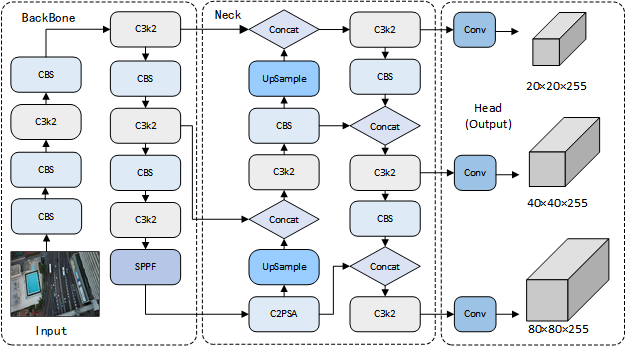
\includegraphics[width=0.8\linewidth]{../figure/yolov11.png}
    }
    \captionsetup{font=footnotesize}
    \bicaption{GAN 网络结构框架}{YOLOv11 network structure diagram.}
    % \label{fig:YOLOv11}
\end{figure}

\begin{figure}[htb]
    \centering
    \subfloat{
    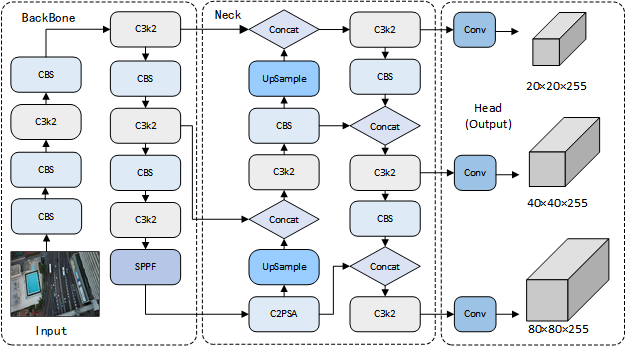
\includegraphics[width=0.8\linewidth]{../figure/yolov11.png}
    }
    \captionsetup{font=footnotesize}
    \bicaption{CycleGAN 网络结构框架}{YOLOv11 network structure diagram.}
    % \label{fig:YOLOv11}
\end{figure}

GAN 通常需要大量的成对数据进行训练,这在许多实际应用中是一个巨大的挑战。例如,在去雾还原任务中,获取大量成对的有雾图像和对应的无雾图像是非常困难的,因为无雾图像往往难以直接获得,或者需要在特定条件下拍摄,这限制了 GAN 在该领域的应用。而 CycleGAN 则可以在无监督的情况下进行训练,即不需要成对的图像数据。它利用循环一致性约束,在只有两个不同域的非配对图像集合的情况下,学习图像之间的映射关系,这大大降低了数据获取的难度,为去雾还原等任务提供了更灵活的解决方案。

GAN 的网络结构相对简单,主要由一个生成器和一个判别器组成。生成器的目标是将随机噪声生成逼真的样本,判别器则用于区分生成样本和真实样本。GAN 的训练目标主要是通过最小化对抗损失函数,使生成器生成的样本尽可能接近真实数据分布,判别器尽可能准确地辨别真假样本。
CycleGAN 的网络结构更为复杂,包含两个生成器和两个判别器。其训练目标不仅包括对抗损失,还包括循环一致性损失。对抗损失确保生成器生成的图像在目标域中具有逼真的外观,而循环一致性损失则保证图像在转换过程中内容的完整性。这种双重约束机制使得 CycleGAN 能够在没有成对数据的情况下,学习到更稳定、更准确的图像转换映射关系。

\subsubsection{生成器网络}

%% 介绍 编码器 - 解码器 结构

CycleGAN是一种用于无监督图像到图像翻译的生成对抗网络架构。其生成器是整个网络的核心组件之一,主要承担着将输入图像从一个域(如雾天图像域)映射到目标域(如无雾图像域)的关键任务。生成器的目标是学习输入图像与目标图像之间的复杂非线性映射关系,使得生成的图像在视觉效果和语义信息上尽可能接近真实的目标域图像,从而实现图像的去雾还原等操作。

CycleGAN 的生成器通常采用编码器 - 解码器结构作为基础框架。编码器部分负责将输入图像逐步下采样,提取图像的多尺度特征。例如,在处理一张雾天图像时,编码器通过一系列卷积层和池化层操作,将图像的空间分辨率降低,同时增加特征图的通道数。这一过程能够捕捉到图像中的局部和全局特征,如雾天图像中的物体轮廓、颜色分布等信息。这些特征对于后续的图像生成至关重要,因为它们包含了生成无雾图像所需的关键语义信息。

解码器部分则与编码器相反,它将编码器提取到的特征逐步上采样,恢复图像的空间分辨率。在上采样过程中,解码器通过转置卷积等操作,将低分辨率的特征图逐步放大,最终生成与输入图像尺寸相同的输出图像。这个过程需要合理地利用编码器提取的特征,以确保生成的图像具有清晰的结构和细节。


%% 介绍ResNet残差块

为了提高生成器的性能,CycleGAN 在编码器 - 解码器结构中加入了残差块。残差块是深度残差网络(ResNet)中的重要组成部分,其核心思想是通过引入 shortcut connection(捷径连接)来缓解深层网络训练中的梯度消失问题。在生成器中,残差块使得网络能够更容易地学习到输入与输出之间的残差映射,而不是直接学习原始映射。

例如,在生成器的中间部分,多个残差块可以堆叠在一起。每个残差块包含两个卷积层和一个 ReLU 激活函数。输入特征先进入第一个卷积层进行卷积操作,然后通过 ReLU 激活函数引入非线性,接着进入第二个卷积层。最后,将第二个卷积层的输出与输入特征相加,得到残差块的输出。这种设计使得网络在训练过程中能够更有效地传播梯度,从而能够构建更深的生成器网络,以捕捉更复杂的图像特征和映射关系。

%% 卷积与反卷积

卷积层是生成器中的基础组件,用于提取图像的局部特征。在编码器部分,卷积层通过卷积核在图像上滑动,进行加权求和操作,提取图像的边缘、纹理等特征。卷积层的输出通道数通常会逐渐增加,以捕捉更丰富的特征信息。

反卷积层(或转置卷积层)在解码器部分用于上采样操作,将低分辨率的特征图逐步放大。反卷积层通过学习卷积核的反向操作,将特征图的空间分辨率提高,从而恢复图像的细节。在反卷积过程中,合理的参数设置和初始化对于生成图像的质量至关重要。



\subsubsection{判别器网络}

全局判别器在整个图像层面进行判断,关注图像的整体特征和分布。它接收完整的图像作为输入,通过多层卷积操作提取图像的全局特征,包括图像的整体结构、颜色分布、纹理模式等宏观信息。其主要作用是判断输入图像是否符合目标域图像的整体特征分布,确保生成图像在整体上具有真实图像的外观和风格。例如,在去雾任务中,全局判别器会学习雾天图像和清晰图像在整体上的差异,如雾天图像通常具有较低的对比度、偏白的颜色倾向以及模糊的轮廓等特征,从而指导生成器生成具有清晰结构、自然颜色分布和高对比度的去雾图像。

全局判别器通常采用卷积神经网络(CNN)结构,包含多个卷积层、激活函数层(如 Leaky ReLU)以及池化层。输入图像经过卷积层的逐层特征提取,图像的空间尺寸逐渐减小,而特征通道数逐渐增加,最终得到一个特征向量。该特征向量被送入全连接层,输出一个概率值,表示输入图像属于目标域真实图像的概率。在训练过程中,全局判别器与生成器进行对抗训练。生成器试图生成能够欺骗全局判别器的图像,使其误认为生成图像是真实图像;而全局判别器则不断学习如何更准确地区分真实图像和生成图像,通过梯度下降更新网络参数,优化判别性能。这种对抗训练过程促使生成器不断提升生成图像的整体质量,使其在全局特征上逐渐接近真实图像的分布。

%% 全局判别器

全局判别器在去雾过程中发挥着关键作用。它能够确保去雾后的图像在整体上具有清晰、自然的视觉效果,避免出现整体结构失真或颜色偏差等问题。例如,当生成器生成的去雾图像整体对比度较低或颜色偏暗时,全局判别器会给出较低的真实性概率,从而促使生成器调整生成策略,提高去雾图像的整体质量。通过全局判别器的监督,生成器能够生成符合清晰图像全局特征的去雾结果,增强去雾图像的视觉吸引力和可用性。


局部判别器聚焦于图像的局部区域,关注图像的细节特征和局部纹理。它通过随机裁剪或采样等方法获取图像的局部小块区域作为输入,对这些局部区域进行判别。其主要作用是确保生成图像在局部细节上具有真实图像的纹理和结构特征,避免生成图像出现模糊、失真或不合理的局部图案。在去雾任务中,局部判别器能够帮助生成器恢复图像中被雾气遮挡的细节信息,如物体的边缘、纹理等,使去雾后的图像在局部区域更加清晰、真实。

局部判别器的网络结构与全局判别器类似,也是基于 CNN 构建。由于其输入是图像的局部小块区域,因此网络的层数和参数量相对较少。局部判别器对输入的局部区域进行卷积操作,提取局部特征,如边缘、纹理、局部颜色过渡等细节信息。经过多层卷积和激活函数处理后,输出一个概率值,表示该局部区域属于目标域真实图像对应局部区域的概率。在训练过程中,局部判别器同样与生成器进行对抗训练。生成器需要生成在局部细节上逼真的图像,以欺骗局部判别器;而局部判别器则不断学习如何更准确地辨别局部区域的真实性。这种对抗训练使得生成器在生成图像时更加注重局部细节的还原和真实感,提高了去雾图像的细节质量。

%% 局部判别器

局部判别器对于去雾效果的提升主要体现在图像细节的恢复和增强方面。在雾天图像中,物体的边缘和纹理往往被雾气模糊,细节信息丢失严重。局部判别器能够指导生成器在去雾过程中有效地恢复这些局部细节,使去雾后的图像能够呈现出物体清晰的轮廓和丰富的纹理。例如,对于建筑物的窗户、树叶的脉络等细节部位,局部判别器可以促使生成器生成更加精细、真实的细节,从而提高去雾图像的整体质量和视觉效果。同时,局部判别器还有助于避免生成图像出现局部失真或不合理的人工痕迹,确保去雾图像的自然性和可信度。


全局判别器和局部判别器在 CycleGAN 的去雾还原算法中相互补充、协同作用。全局判别器从整体上把握图像的宏观特征和风格,确保生成图像在整体布局、颜色分布等方面符合清晰图像的要求;局部判别器则专注于图像的细节部分,保证生成图像在局部区域具有真实的纹理和结构。在训练过程中,生成器需要同时满足全局判别器和局部判别器的要求,既要生成具有真实整体特征的图像,又要在局部细节上做到逼真自然。这种协同作用使得生成器能够生成高质量、高保真的去雾图像,有效地解决了图像去雾中的细节恢复和整体质量提升的难题。例如,在处理一幅包含复杂场景的雾天图像时,全局判别器确保整个场景的清晰度和自然度,如天空的蓝色、地面的颜色分布等;局部判别器则负责恢复场景中物体的细节,如人物的面部表情、车辆的标志等,从而使最终的去雾图像在整体和局部都达到较好的效果。

\subsection{优化的CycleGAN网络}

\subsubsection{Transformer模块}

\subsubsection{改进的生成器网络}

\subsubsection{优化的损失函数}


\subsection{去雾还原实验结果和分析}

\subsubsection{数据集}

\subsubsection{实验环境}

\subsubsection{实验结果和分析}


\subsection{本章小结}


% Please add the following required packages to $y$our document preamble:
% \usepackage{booktabs}
